\chapter{Implementation Overview}
\label{Chapter3}
\section{Goal of the project}
The scope of this project is to design a vulnerable hardware device, in which the fault is to be discovered by each participant alone. Such weakness gets triggered only when a specific combination of inputs is provided, making the whole design partially functional.
The player can thus report either the actual flag itself (i.e. a numerical value) or a coincise description of his discoverings, in order to be declared as the winner.
\section{Architecture overview}
The top-level Block Cipher includes a LFSR, an ALFSR, a 1-bit adder with support for the carry bit and some additional logic aimed at increasing the complexity of the whole process.
The plaintext is scanned serially by the LFSR, while the seed to the ALFSR is given by the user in a parallel fashion.
\begin{figure}[!ht]
\vspace{0.5cm}
\centering
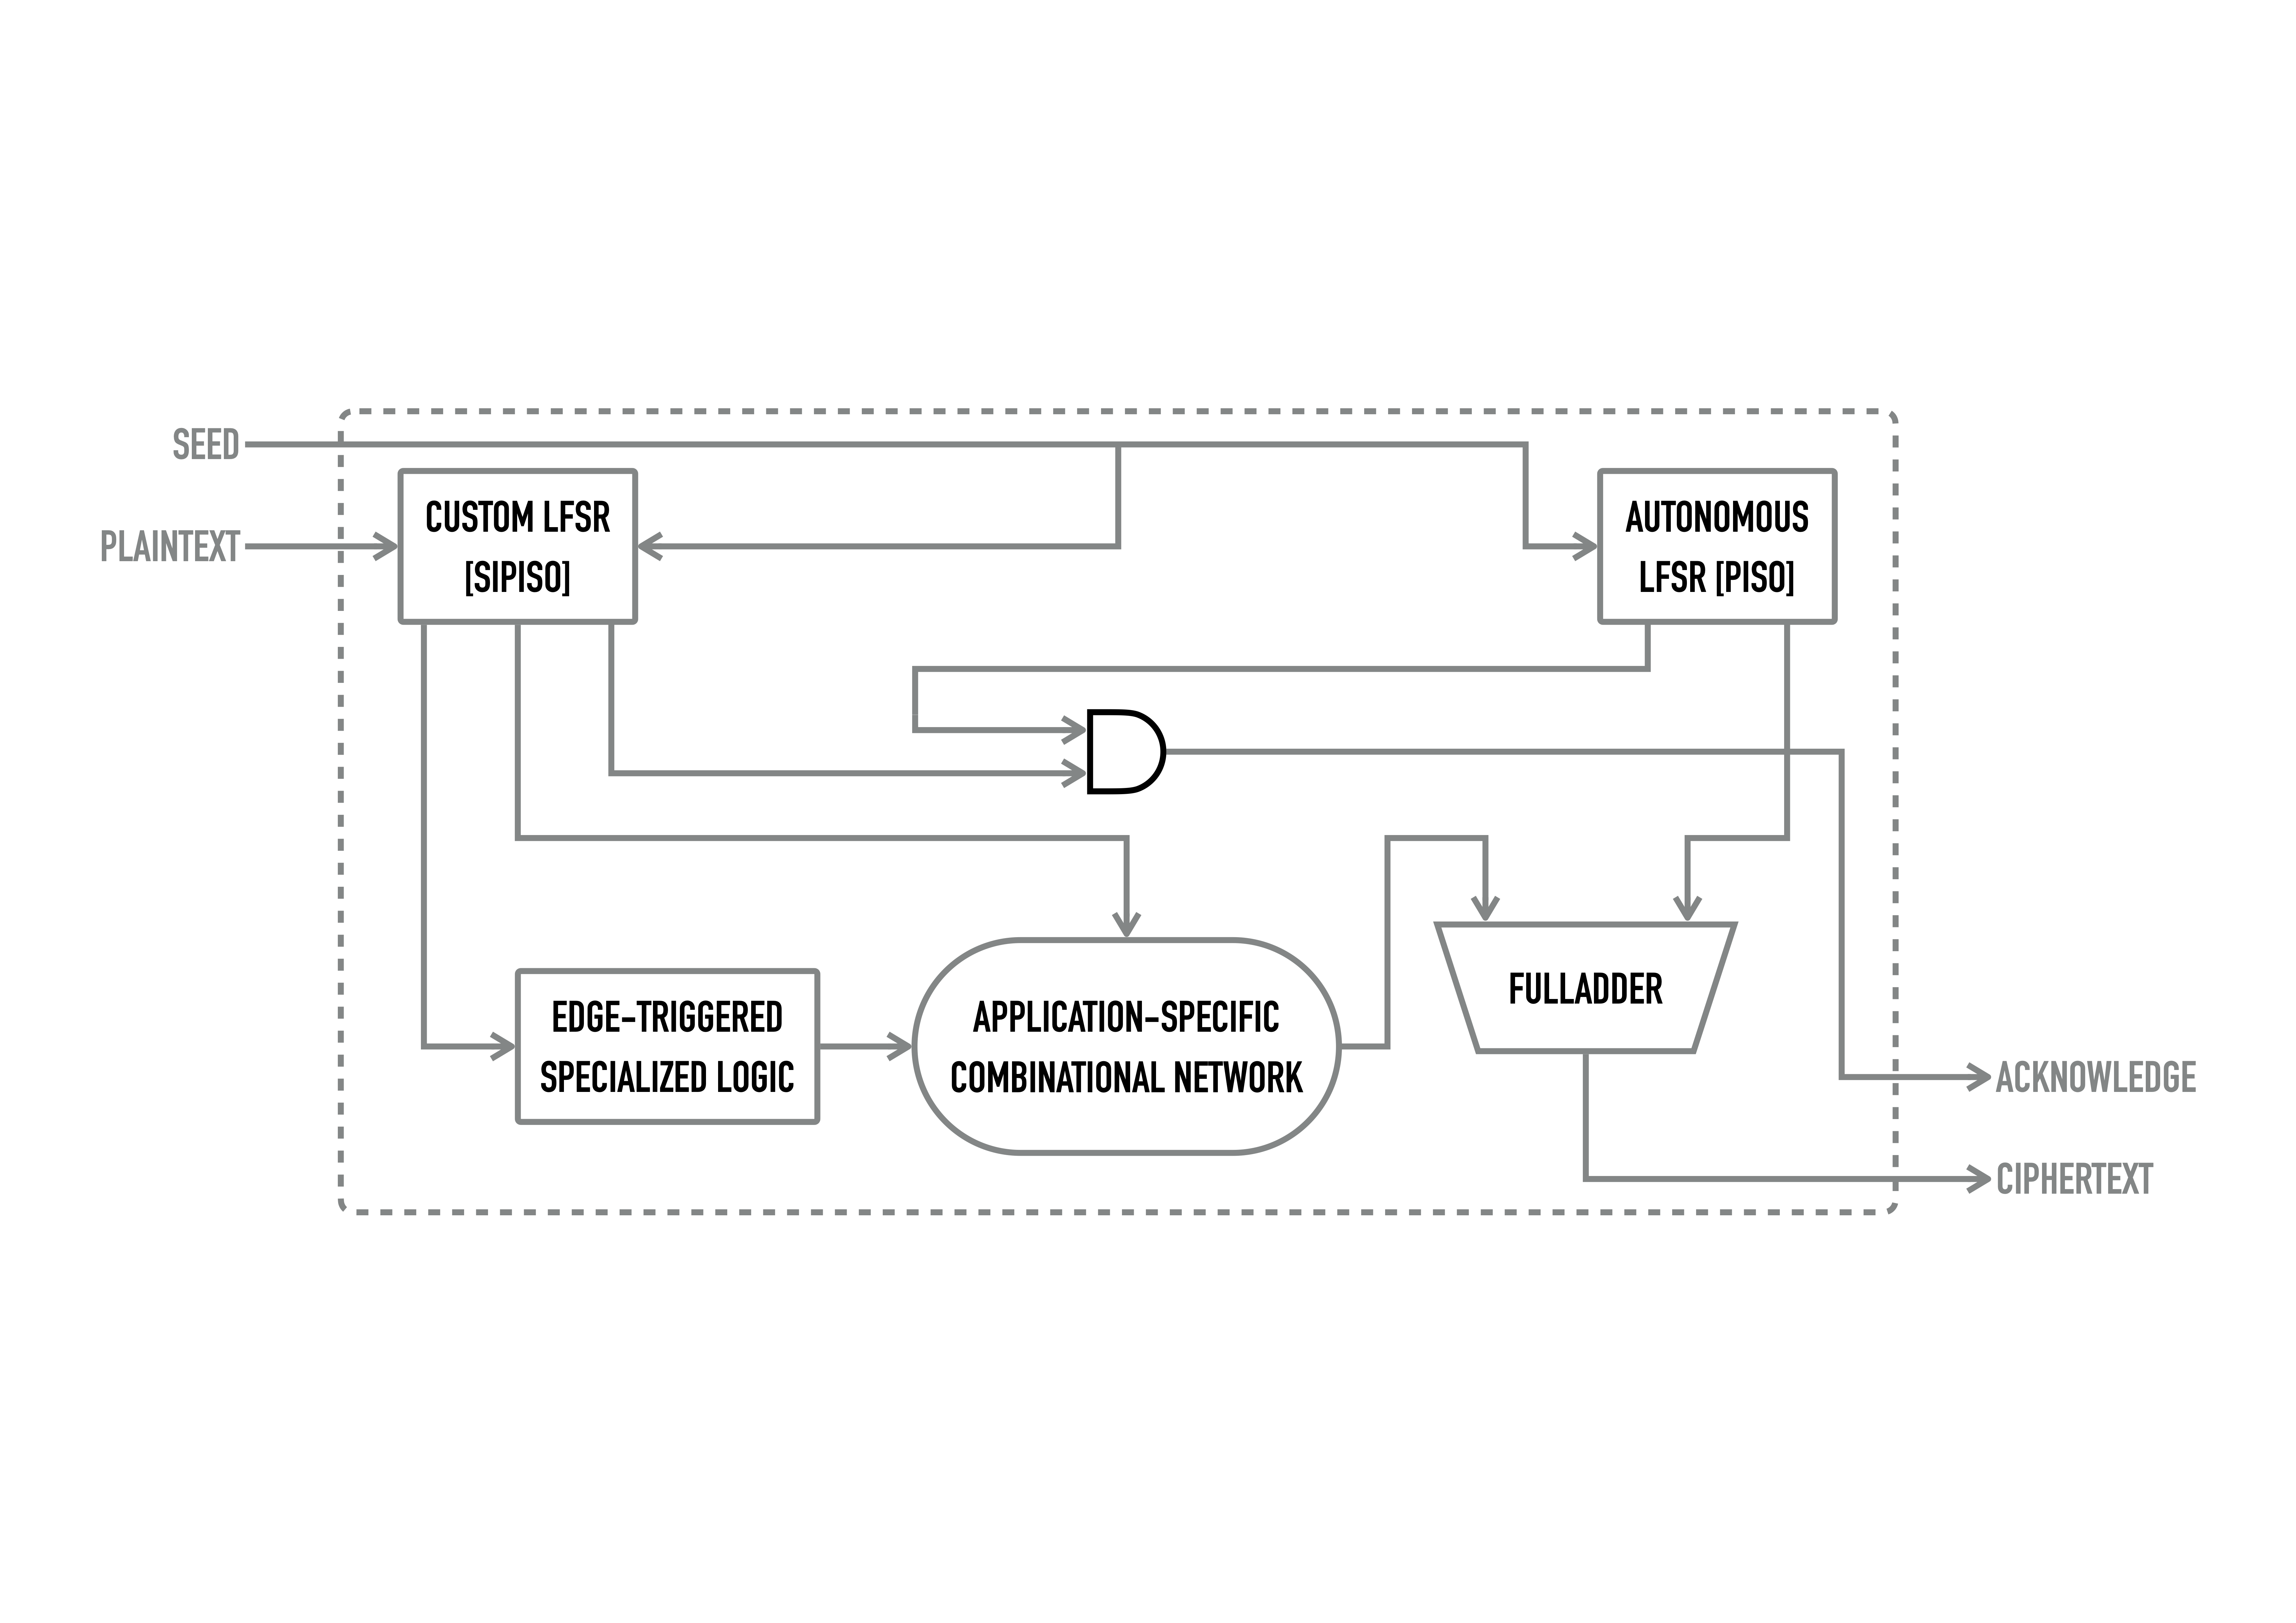
\includegraphics[width=0.75\textwidth]{images/Schematic.png}
\caption{High-level schematic of the design.}
\end{figure}
Each bit coming out of the former register is added to the output of the other one, resulting in the final chipertext. The ackowledge signal is used in conjunction in order to report its validity (after the initialization of the device).

The main takeaway in this context is that the LFSR is indeed a cipher just by itself, as it does perform pseudo-random number generation based on its inputs, but its computations are perfectly linear, as they just involve XOR operations.
Thanks to the contribution of the carry, it's immediately possible to insert a crucial non-linearity that ends up making the entire function irreversible, hence not trivial anymore.
\section{Hardware platform}
\begin{figure}[!ht]
\vspace{0.5cm}
\centering
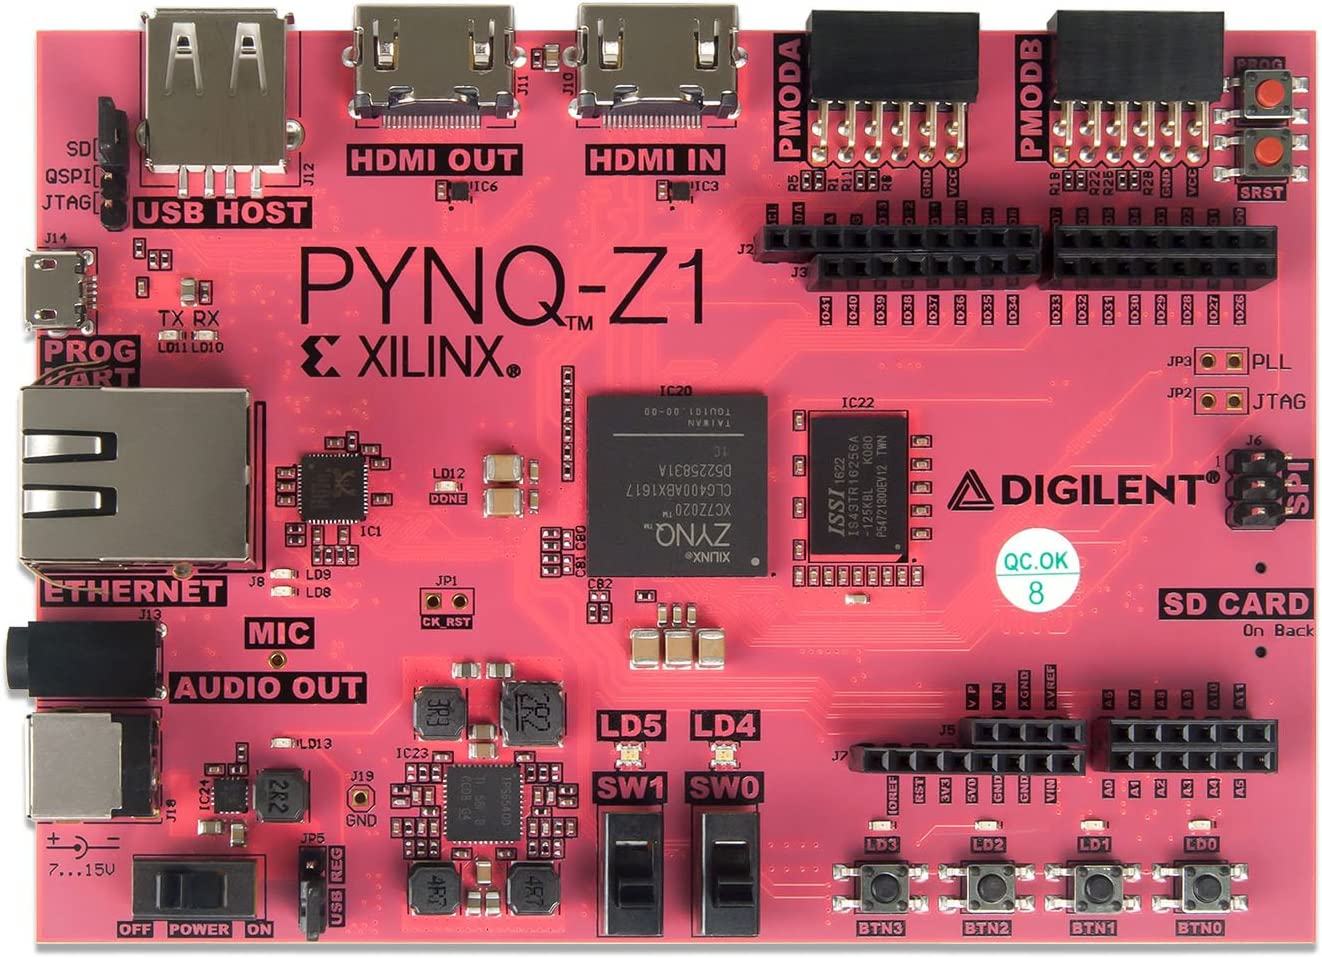
\includegraphics[width=0.75\textwidth]{images/PYNQ.jpg}
\caption{A PYNQ-Z1 Python Productivity board.}
\end{figure}
The design was implemented and tested on a PYNQ embedded board, equipped with a programmable logic equivalent to the Artix-7 FPGA and also a Cortex-A9 processor.
The latter can run Python code that interacts with the Block Cipher, exposing the related functionalities as convenient APIs by means of dedicated libraries.

As the PYNQ also includes an ethernet port, it was possible to create a web server that could offer the challenge online by means of a predefined IP address, which returns the end-product: an interactive webpage.